\chapter{Einseitiges PDF einbinden}
Es ist möglich, PDF als Grafiken einzubinden. Hier ein Beispiel:
\begin{figure}[H]
    \centering
    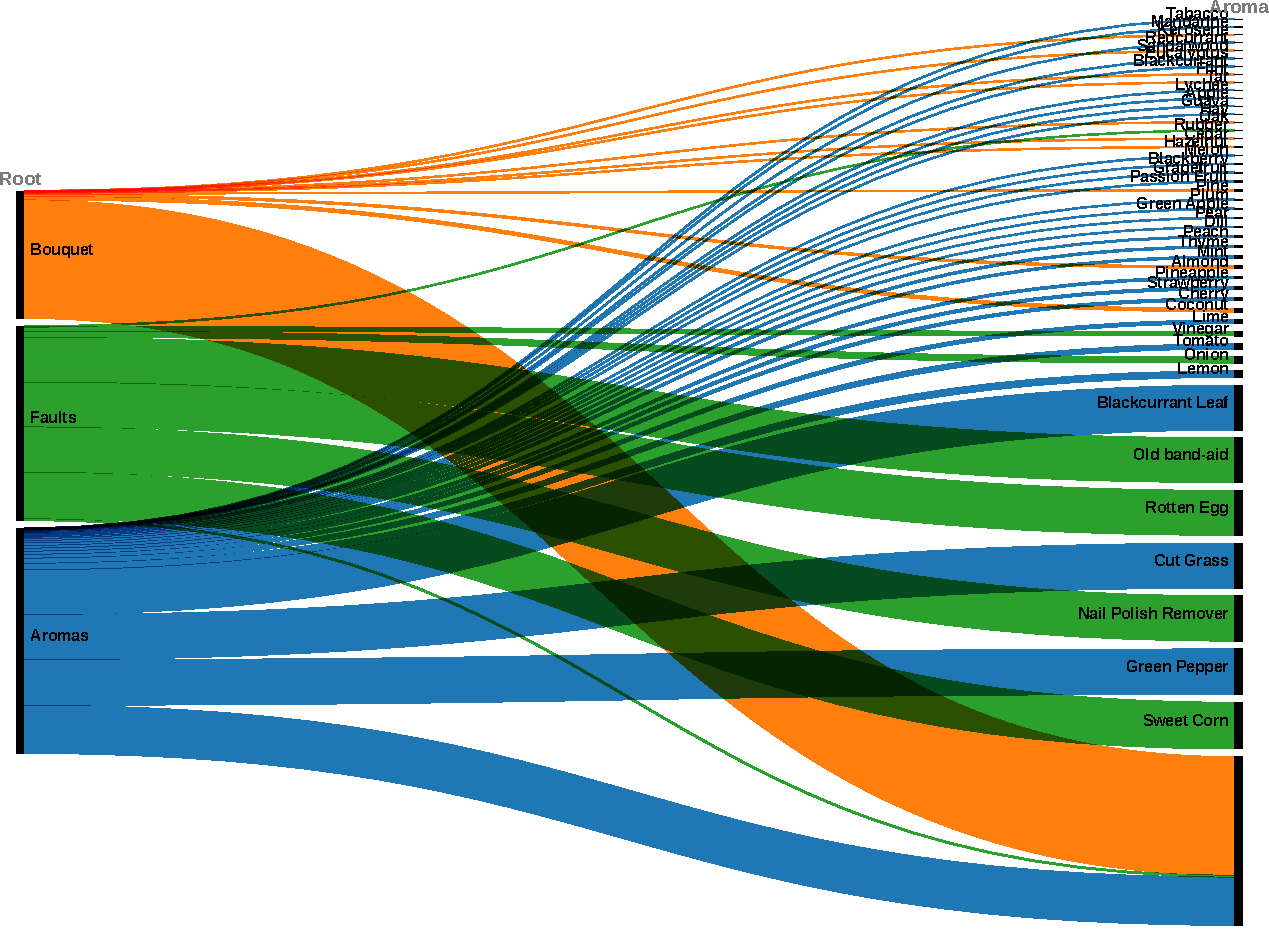
\includegraphics[width=\textwidth]{content/00_assets/example.pdf}
    \caption{Beispiel für Einbindung von PDF-Dateien}
    \label{fig:enter-label}
    \note{Grafik von https://www.rawgraphs.io/}
\end{figure}

\chapter{Mehrseitiges PDF einbinden}
Das Einbinden mehrseitiger PDF ist mittels des \lstinline{pdfpages} Pakets\footnote{https://www.ctan.org/pkg/pdfpages} möglich. Mit dem folgenden Befehl werden die Seiten 9, 15, 25 und 48-50 aus dem books-of-bread PDF eingebunden \parencite{simmons_book_1903}: \\
\lstinline|
\includepdf[pages={9,15,25,48-50}]{content/00_assets/book-of-bread.pdf}|


\includepdf[pages={9,15,25,48-50}]{content/00_assets/book-of-bread.pdf}